% ********** Chapter 1 **********
\chapter{Grundlagen}
\label{sec:background}

Dieses Kapitel stellt bereits vorhandene Technologien vor, welche f"ur die L"osung der Aufgabenstellung relevant sind.
Weiterhin werden Technologien angesprochen, die alternative L"osungen darstellen k"onnten, in diesen F"allen wird kurz
darauf eingegangen, warum sie keine Verwendung finden. Weiterhin werden Begrifflichkeiten f"ur den weiteren Verlauf
des Dokumentes eingef"uhrt und erkl"art.

\section{Common Gateway Interface - CGI}
TODO: bla cgi bla fastcgi bla module

\section{Serviceorientierte Architektur - SOA}
\label{sec:background:soa}
Der Begriff Serviceorientierte Architektur oder englisch Service Oriented Architecture, auch diensteorientierte Architektur,
beschreibt ein Softwarearchitekturkonzept welches versucht durch lose Koppelung autarker Module - sogenannter Services -
Gesch"aftsprozesse besser und schneller abbilden zu k"onnen als traditionelle Architekturen. Diese Services bilden
einzelne Schritte der Gesch"aftsprozesse nach und bieten standardisierte Schnittstellen "uber welche sie angesprochen
werden k"onnen. Dienste werden vom einem \emph{service provider} angeboten und von einem \emph{service consumer}
mittels eines \emph{service request} angesprochen, der Dienst antwortet mittels eines \emph{service response}.
Die Koppelung mehrerer Dienste wird "uber ein oder mehrere Protokolle wie zum Beispiel \emph{SOAP} (siehe \ref{sec:background:soap})
oder \emph{RMI} (siehe \ref{sec:background:rmi}), aber auch durch den Einsatz ganzer dienstorientierter Technologien
wie \emph{CORBA} oder \emph{Enterprise Java Beans} erreicht. 
Aufgrund der Platformunabh"angigkeit solcher Technologien eigenet sich ein solche Architektur auch besonders vorhandene
Strukturen miteinander zu verbinden.
Ein weiterer wesentlicher Aspekt von SOA ist die Kapselung des Zugriffes
auf persistente Daten durch einzelne Services, welche als einzige schreibend auf diese Daten zugreiffen k"onnen, was 
die Gew"ahrleistung der Konsitenz solcher persistenter Daten erheblich vereinfacht. 

\section{Skriptsprachen}
\label{sec:background:script}

Als Skriptsprachen bezeichnet man Programmiersprachen, welche urspr"unglich vor allem zur L"osung
kleinerer Programmieraufgaben entwickelt wurden. Sie stellen im Allgemeinen keine so hohen formalen 
Anspr"uche an den Programmierer wie "'vollst"andige"' Programmiersprachen, so verzichten sie
beispielsweise oft auf den Deklarationszwang von Variablen. Weitere Merkmale die h"aufig bei
Skriptsprachen anzutreffen sind sind unter anderem die dynamische beziehungsweise oft auch komplett 
fehlende Typisierung von Variablen, die automatische Speicherverwaltung und vor allem das
"ubersetzungsfreie Ausf"uhren - sprich die Skripte werden "'interpretiert"'. Dies f"uhrt allerdings
dazu, dass Skriptsprachen oft nicht so effizient sind wie direkt "ubersetzte Programme, und dazu
dass viele Fehler welche ein Compiler finden beziehungsweise komplett verhindern w"urde erst zur
Laufzeit und somit m"oglicherweise im Produktivbetrieb auftreten.
Der "Ubergang zwischen klassischen Programmiersprachen und Skriptsprachen ist heute fliessend, so 
bieten Sprachen wie beispielsweise Java auch eine automatisierte Speicherverwaltung und werden nicht
direkt in Maschinencode sondern in Bytecode "ubersetzt welcher dann interpretiert wird, w"ahrend 
Skriptsprachen wie Python oder Ruby teilweise sehr hohe formale Anspr"uche stellen und sehr robust sind.
Die klassischen Einsatzgebiete von Skriptsprachen werden heute erweitert durch Webanwendungen und
\emph{rapid prototyping}, auch werden sie gerne als sogenannte \emph{glue languages} - als 
verbindender "'Kleber"' zwischen verschiedenen Systemen, Programmen und Programmiersprachen -
eingesetzt. Skriptsprachen sind ausserdem beliebt um Softwaresysteme f"ur weniger versierte Anwender
leicht erweiterbar zu machen, indem sie eine kontrollierte, leicht erlernbare und trotzdem 
ausreichend m"achtige Umgebung bieten.
Im weiteren Verlauf dieses Dokumentes werden Programme, welche in einer Skriptsprache geschrieben sind 
auch kurz als "'Skripte"' bezeichnet.

\subsection{PHP}
\label{sec:background:php}

Das PHP-Manual \cite{PHPMAN} schreibt "uber PHP: "`PHP (Akronym f"ur "'PHP: Hypertext Preprocessor"') 
ist eine weit verbreitete und f"ur den allgemeinen Gebrauch bestimmte Open Source Skriptsprache, 
welche speziell f"ur die Webprogrammierung geeignet ist, und in HTML eingebettet werden kann."'

Das heutige PHP entstand aus den urspr"unglich 1994 von \emph{Rasmus Lerdorf} in C geschriebenen und "uber CGI
ausgef"uhrten "'Personal Home Page Tools"'. 1995 wurden diese von Lerdorf erstmals als "'PHP/FI"' ver"offentlicht,
nachdem er sie mit einem Interpreter f"ur Formulardaten ausgestattet hatte.
1997 schrieben die beiden israelischen Entwickler \emph{Zeev Suraski} und \emph{Andi Gutmans} den Parser neu und
schufen so die Grundlage f"ur PHP 3, welches 1998 erstmals ver"offentlicht wurde. Diese Version bot auch 
erstmals grundlegende M"oglichkeiten zur objektorientierten Programmierung, allerdings war die gesamte 
Standardbibliothek noch prozedural angelegt.
Suraski und Gutmans fingen daraufhin an den Kern von PHP neu zu schreiben, welcher seit 1999 als \emph{Zend Engine}
von der neu gegr"undeten \emph{Zend Technologies} vertrieben wird. Im Mai 2000 wurde PHP 4 der
"Offentlichkeit als erstes PHP vorgestellt, welches die Zend Engine in der Version 1.0 nutzte (siehe auch \cite{ZENDENGINE}).
PHP 4 wird bis heute von Zend supported und wird bei 1\&1 noch produktiv eingesetzt, obwohl es noch sehr unter den
mangelhaften F"ahigkeiten zur Objektorientierung von PHP 3 leidet, so werden weder Kapselung der Daten durch 
zum Beispiel private Variablen, noch Destruktoren oder Fehlerbehandlung "uber Exceptions unterst"utzt.
July 2004 wurde PHP 5 zusammen mit der Zend Engine II ver"offentlicht und bot endlich lang erwartete Features wie
robuste Objektorientierung, native SOAP-Unterst"utzung (siehe \ref{sec:background:soap}), 
Iteratorkonstrukte und Exceptions. Zu diesem Zeitpunkt wird an der n"achsten PHP Version 6 entwickelt, diese
befindet sich allerdings noch in einem sehr fr"uhen Stadium, so wird noch heftig "uber die Richtung
debatiert in welche sich PHP in Zukunft bewegen soll.\\
PHP Quellcode wird - wie bei vielen Skriptsprachen, zum Beispiel Perl - nicht kompiliert sondern zur Laufzeit ausgewertet und interpretiert.
Die Sprache bietet nur einige wenige Datentypen, welche alle in einer einzigen Art von Variable gespeichert werden 
(\emph{weak typing}) - sprich Variablen k"onnen zur Laufzeit ihren Typen "aendern, was von vielen als ein weiterer
Kritikpunkt angesehen wird da es zu Laufzeitfehlern kommen kann die in anderen Sprachen schon von vorneherein 
ausgeschlossen sind. Ein weiteres Problem ist dass der Sprachumfang von PHP durch Dritte mittels \emph{Extensions}
genannter Erweiterungen erweitert werden kann und auch wird. Dies muss allerdings zur Kompilierzeit von PHP geschehen, was wiederum
dazu f"uhrt dass verschiedene PHP-Installationen auch verschiedenen Funktionsumfangs sein k"onnen, und dazu dass
verschiedene Extensions "'gleichen Typs"' - zum Beispiel die Datenbankerweiterungen zu MySQL und Sybase - nicht
nur unterschiedliche Methodensignaturen, sondern auch unterschiedliches Verhalten "ahnlicher Methoden haben.
Der Einsatz von PHP innerhalb von 1\&1 ist historisch vor allem dadurch zu erkl"aren, dass es zun"achst keine 
konkurrenzf"ahigen Technologien gab, und sp"ater erstens schon sehr viel in diese Technologie investiert
worden war und zweitens etwaiige technischen Nachteile von PHP durch im Unternehmen vorhandenes Know-How sehr gut
ausgeglichen werden konnten.


\section{XP-Framework}
\label{sec:background:xp}

Das XP-Framework \cite{XPHP} (XP) ist der Hauptgrund warum - trotz der sehr mangelhaften M"oglichkeiten zur 
Objektorientierung - bei 1\&1 noch haupts"achlich PHP 4 eingesetzt wird. XP ist ein modulares Framework welches
dem Anwender das Entwickeln jeglicher Anwendung in PHP erleichtern soll, es wird seit 2001 nach streng 
objektorientierten Kriterien und mittels eines agilen Prozesses haupts"achlich bei 1\&1 hausintern entwickelt,
ist aber komplett open source und wird unter der \emph{BSD licence} \cite{BSDLICENCE} vertrieben.
Eine zentrale Motivation f"ur die Entwicklung des XP-Frameworks war das "uberwinden der angesprochenen
Defizite von PHP 4, so wurde unter anderem ein eigener Exception-Mechanismus, Methoden zum dynamischen
Laden und zur Reflektion von Klassen, OO-Mapping von Datenbankzugriffen, sowie Abl"aufe zur sauberen 
Trennung von Logik und Pr"asentation entwickelt, desweiteren enth"alt XP "Aquivalente zu so gut wie allen Klassen 
der Java Foundation Classes.
Durch saubere, an Javadoc \cite{JAVADOC} angelehnte Dokumentation im Sourcecode wird versucht die mangelnde
Typisierung in PHP zu "uberwinden, was M"oglichkeiten zur automatischen Generierung von API-Dokumentation und zum
Beispiel WSDLs \cite{WSDLSPEC} f"ur SOAP er"offnet.
Alles in allem erlaubt das XP-Framework die Vorteile von PHP wie kurze Entwicklungszeiten und einfache 
Programmierung zu nutzen ohne auf die Vorteile der Objektorientierung zu verzichten.
Viele diese Funktionen setzen allerdings vorraus, dass das ausf"uhrende PHP bestimmte Extensions bereitstellt,
ohne welche beispielsweise das Transformieren von XML mittels XSL, die FTP- und Mailfunktionalit"at oder auch
der Zugriff auf Datenbanken wie MySQL oder Sybase nicht m"oglich w"aren.
Eine Portierung des Frameworks nach PHP 5 wird zwar schon l"anger geplant, allerdings gestaltet sich dieses 
aufgrund der ge"anderten Verhaltensweisen der Programmiersprache bez"uglich Referenzen sowie die von den PHP-Entwicklern
etwas unbedacht eingef"uhrten Exceptions schwierig. Desweiteren werden PHP st"andig neue Standardklassen
hinzugef"ugt was ob der fehlenden Namensr"aume zu Kollisionen mit Klassen des Frameworks f"uhrt.


\section{SOAP}
\label{sec:background:soap}
SOAP (urspr"unglich stehend f"ur \emph{\textbf{S}imple \textbf{O}bject \textbf{A}ccess \textbf{P}rotocol})
ist ein Protokoll welches den Austausch XML-basierter Nachrichten "uber ein Rechnernetzwerk - "ublicherweise
mittels HTTP - erlaubt. SOAP-Implementierungen sind heute f"ur fast jede Programmiersprache verf"ugbar, so wird es
ab PHP Version 5 nativ unterst"utzt, und auch innerhalb des XP-Frameworks stehen entsprechende Klassen zur Verf"ugung.
SOAP entstand aus einer Zusammenarbeit von \emph{Dave Winer} und \emph{Microsoft}, im Jahre 2000 schlossen sich 
weitere Firmen, darunter IBM, der Entwicklungsgruppe an und reichten den Entwurf zu SOAP 1.1 beim 
\emph{World Wide Web Consortium} (W3C) zur Weiterentwicklung ein, welches 2003 den aktuellen Standard SOAP 1.2
ver"offentlichte.
Eine SOAP Nachricht besteht lediglich aus einem \emph{SOAP-Envelope} welcher wiederum ein (optionales) \emph{Header}-Element
und ein \emph{Body-Element} enth"aelt und verwendete Namesr"aume festlegt \cite{SOAPSPEC}. Die eigentlichen Nutzdaten sind
im Body-Element untergebracht und m"ussen vom Empf"anger der Nachricht intepretiert werden, w"ahrend im Header-Element Metadaten
zur Nachricht enthalten sind, welche ebenfalls von den empfangenden Stationen intepretiert werden m"ussen. Diese sehr schmale
Spezifikation erlaubt es sehr flexible Anwendungen zu entwickeln, allerdings bringt SOAP auch einige Nachteile mit sich:\\
Aufgrund der Verwendung von XML zur Kodierung der zu "ubertragenden Informationen vervielfacht sich das "Ubertragungsvolumen
deutlich - in manchen F"allen um bis zu 125\% - was nicht nur Probleme mit der verwendeten Bandbreite verursacht, sondern auch
erhebliche Mengen an Rechenleistung bei der Generierung und Verarbeitung der Nachrichten erfordert. Ein weiterer Kritikpunkt ist
die mangelhafte und zum Teil sich selbst widersprechende Spezifikation selbst, was unter anderem dazu f"uhrt dass mittels verschiedener
Software (\emph{tool-chains}) erzeugte SOAP-Services und -Anwendungen nicht ohne h"andisches Eingreiffen des Entwicklers miteinander kommunizieren 
k"onnen.
Da der Standard keine Aussagen "uber Transaktionalit"at trifft m"usste solches Verhalten - falls gew"unscht - von jeder Applikation selbst
definiert und vom Benutzer implementiert werden, was dazu f"uhrt dass es in der Praxis unm"oglich ist Anwendungen mittels SOAP zu
verwirklichen welche Transaktionen ben"otigen w"urden. Auch existiert kein Standard der es erlaubt dynamisch Daten "uber an einem Ort verf"ugbare
Dienste zu erlangen. Zu diesem Zweck wird meist ein \emph{WSDL}-Dokument \cite{WSDLSPEC} eingesetzt, allerdings wird auch an diesem
Standard viel Kritik ge"ubt, so spezifiziert er beispielsweise weder wie ein WSDL-Dokument f"ur einen speziellen Dienst zu beziehen ist,
noch enth"alt ein solches Dokument Informationen die "uber die Syntaktische Beschreibung des Dienstes hinausgehen.
Ein weiteres SOAP-spezifisches Problem ist,
dass kein Mechanismus definiert wird "uber welchen Nachrichten aktiv an einen Anwender "ubermittelt werden k"onenn, we\ss halb dieser
st"andig "uberpr"ufen muss ob neue Daten f"ur ihn anliegen ("'Polling"').

\section{XML-RPC}
\label{sec:background:xmlrpc}
XML-RPC (vom englischen \textbf{R}emote \textbf{P}rocedure \textbf{C}all) ist ein Vorg"anger von SOAP, und setzt - wie schon
aus dem Namen hervorgeht - ebenfalls XML zur Kodierung der zu "ubertragenden Daten ein. Im Gegensatz zu den meisten anderen
Sytemen die den Aufruf entfernter Methoden erlauben ist XML-RPC sehr simpel gehalten und definiert nur einige wenige
Datentypen. Diese sehr schlanke Spezifikation verhindert zwar dass die zu "ubertragenden Nachrichten wie bei SOAP zu sehr 
aufgebl"aht werden, allerdings schr"ankt sie auch die m"ogliche Komplexit"at der zu versendenden Strukturen stark ein.
XML-RPC eignet sich folglich gut um einfache Dienste anzubieten, f"ur komplexe Anwendungen hingegen w"urde man sich eher 
f"ur eine fortgeschrittenere Technologie entscheiden, nichtsdestotrotz sollte es an dieser Stelle erw"ahnt werden.

\section{Java Enterprise Edition - Java EE}
\label{sec:background:jboss}
\label{sec:background:rmi}
Java EE \cite{JEEHP} erweitert den Java Standard unter anderem um Funktionsalit"at, die es dem Entwickler erlaubt verteilte, transaktionsbasierte und
mehrschichtige (\emph{multitier}) Anwendungen zu entwickeln. Hierzu spezifiziert Java EE mehrere Komponenten, wie unter anderem
\emph{Enterprise Java Beans (EJBs)}, \emph{Servlets} und \emph{Java Server Pages (JSPs)}, und APIs sowie klare Schnittstellen zwischen
diesen Komponenten. Die diese Technologien ben"otigen einen sogenannten \emph{Java Application Server} welcher die n"otige Infrastruktur
f"ur Sicherheit, Transaktionsmanagement, Kommunikation und vielem mehr unabh"angig von Betriebssystem, Netzwerk- und Rechnerarchitektur
bereitstellt. Der Application Server ist in mehrere Module (sogenannte \emph{Container}) unterteilt welche als Laufzeitumgebungen f"ur einzelne
Komponenten fungieren - so werden zum Beispiel EJBs im EJB-Container ausgef"uhrt. Zum Aufruf von Methoden entfernter Objekte bietet Java 
RMI (\textbf{R}emote \textbf{M}ethod \textbf{I}nvocation) an, was entweder "uber ein eigenes Protokoll oder aber "uber IIOP gefahren werden kann.
RMI ist ein bin"ares Protokoll was den Overhead den es erzeugt klein h"alt, ausserdem bietet es Transaktionssicherheit. RMI eignet sich deswegen besser f"ur 
komplexe Anwendungen bei denen auch die Antwortzeit eine Rolle spielt. RMI hat sich auch innerhalb der 1\&1 als bevorzugtes Protokoll 
etabliert um Dienste miteinander zu verkn"upfen, leider existiert keine PHP-Implementation, und die Komplexit"at und die bin"are Natur des
Protokolls machen es fast unm"oglich eine solche selbst zu entwickeln.


\section{Enterprise Application Server Connectivity - EASC}
\label{sec:background:easc}
EASC ist eine haupts"achlich von Christian Gellweiler im Rahmen einer Diplomarbeit f"ur 1\&1 entwickelte 
"'Protokollbr"ucke welche es PHP-Applikationen erlaubt RMI-Aufrufe mittels eines Stellvertreters auszuf"uhren, welcher
Daten und Anweisungen "uber ein generisches Protokoll erh"alt."' \cite{EASC}\\
Dieser Proxy kommuniziert mit dem innerhalb des J2EE-Application-Servers ausgef"uhrten sogenannten \emph{EASC Service-MBean} mittels
eines speziellen Protokolls, welches die Serialisierung und "Ubertragung von Daten und Objekten erlaubt.
Die Erzeugung der Proxyklassen ("'Stub"') "ubernimmt ein spezielles Programm welches es dem Entwickler erlaubt aus einer in Java geschriebenen
Remote Interface Klasse des aufzurufenden Enterprise Beans eine "aquivalente PHP Klasse zu erzeugen.
Wird nun innerhalb von PHP eine Methode des Stubs aufgerufen serialisiert dieser diesen Aufruf und "ubermittelt diesen mittels des EASC-Protokolls
an das MBean. Das MBean deserialisiert diesn, und t"atigt nun die seinerseits n"otigen RMI Aufrufe.
Gegenrichtung werden R"uckgabewerte und Fehlermeldungen - wiederum "uber besagtes Protokoll - zur"uckgeliefert.
EASC erlaubt es also einer komplett in PHP geschriebenen Anwendung auf J2EE-Dienste zuzugreiffen welche andernfalls nur
erreichbar w"aren w"urde diese Anwendung selbst in einer solcher Umgebung ausgef"uhrt. Allerdings bietet EASC keine M"oglichkeit
selbst Dienste in PHP zu entwickeln die ihrerseits aus einer J2EE-Umgebung mittels RMI aufgerufen werden k"onnen.
\begin{figure}[h]
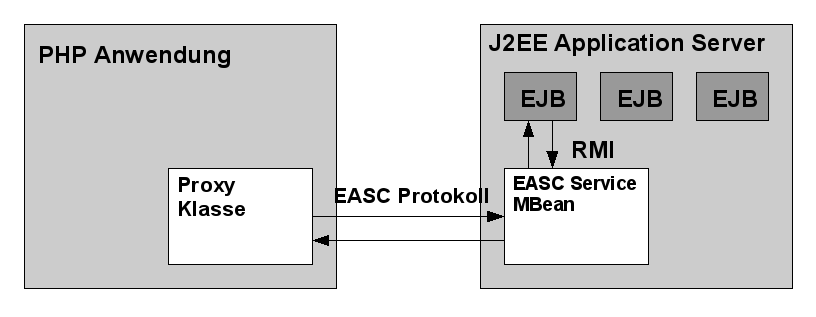
\includegraphics[width=\textwidth]{intro/img/easc.png}
\caption{EASC Funktionsweise - nach \cite{EASC}}
\label{fig:easc}
\end{figure}

\section{Java Native Interface - JNI}
\label{sec:background:JNI}

Java-Programme erreichen ihre Plattformunabh"angigkeit vorrangig dadurch, dass sie eine virtuelle Maschine (\emph{Java Virtual Machine - JVM}) vorraussetzen in welcher sie
ausgef"uhrt werden. Diese virtuelle Maschine verhindert allerdings auch dass beispielsweise plattformspezifische Funktionen oder vorhandene, nicht in Java
geschriebene Programmbibliotheken aus Java heraus angesprochen werden k"onnen.
Um dies zu umgehen bietet Java dem Entwickler mit dem JNI \cite{JNIHP} eine standardisierte M"oglichkeit zur Laufzeit betriebssystemspezifische Bibliotheken 
(.dll unter Windows, .so unter unixoiden Betriebssystemen) einzubinden und Funktionen beziehungsweise Methoden welche diese bereitstellen aufzurufen. 
JNI erm"oglicht nicht nur den Aufruf solcher Methoden aus Java heraus, sondern auch Aufrufe von Java Methoden aus der eingebundenen Bibliothek. 
Native Funktionen werden in einer eigenen .c oder .cpp (C oder C++) Datei implementiert, wobei C++ eine etwas "'sauberere"' Schnittstelle mit dem JNI erlaubt.
Um aus Java heraus eine native Methode aufzurufen muss diese im Javaquelltext als \emph{native} deklariert werden. Aus der kompilierten Java-Klasse kann
mittels des Werkzeuges \emph{javah} eine Headerdatei erstellt werden, die die n"otige Funktionsdeklaration enth"alt. Mit Hilfe dieser Headerdatei kann
nun die native Programmbilbiothek entwickelt werden.
In der Java-Anwendung muss vor dem Aufruf der nativen Methode die entsprechende Programmbibliothek mittels \emph{System.loadLibray} geladen werden.

JNI wird unter anderem f"ur performance-kritische Zwecke (zum Beispiel in Grafikanwendungen) eingesetzt, allerdings setzen auch viele im Java Standard enthaltene
Klassen - wie beispielsweise jene die f"ur die Audioausgabe oder f"ur Dateizugriffe zust"andig sind - JNI Implementierungen vorraus um auf diese
plattformspezifischen Funktionalit"aten in einer sicheren und kontrollierten Art und Weise zuzugreiffen. Leider sichert JNI den Anwender nicht gegen s"amtliche m"oglichen
Fehler ab: zwar kann beim Aufruf der Bibliotheksfunktionen kein Fehler mehr begangen werden, allerdings k"onnen sich Programmierfehler innerhalb der
Bibliothek selbst weiterhin negativ auswirken, und zwar nicht nur auf den nativen Teil der Anwendung, sondern unter Umst"anden sogar auf die JVM selbst.


% ********** End of chapter **********
